%
% Chapter 4
%

\chapter{PHYSICS OBJECTS}
Each of the CMS subdetectors (neglecting the trigger system) technically only record and detect hits and energy deposits. While these hits and energy deposits are almost
always due to passing particles, the detectors and readouts themselves only produce information about the position, value, and multiplicity of
these hits and energy deposits. Thanks to clever and accurate experimental techniques, we reconstruct various particles from these hits and energy deposits.

In part because CMS detects only the hits and energy deposits directly, and the particles are inferred from this information,
reconstructed particles are referred to as physics \emp{objects} in this context.
The reconstruction technique varies greatly with different objects and the subdetectors used to detect and record their hits and energy deposits. 
% Using
%the term particles implies certainty about the identify of the object, and because there is some uncertainty, however small, inherent in the reconstruction, objects is
%more accurate and widely used.

\section{Object Reconstruction and Particle Flow}
The particle flow algorithm is used by CMS to reconstruct physics objects from hits and energy deposits. Particle Flow and CMS are unique in the sense
that nearly all physics analyses performed on data collected by CMS use objects reconstructed with this single algorithm. The primary advantage of this strategy is
uniform and consistent object definitions across nearly all papers published on behalf of CMS. Other collaborations such as ATLAS do not use
the same algorithm collaboration-wide. The purpose of particle flow is to identify all final-state stable particles in an event recorded by CMS, specifically electrons,
mouons, taus, jets and photons. Particle flow optimally combines building-block information (hits and energy clusters) from all subdetectors to reconstruct objects and
determine particle type, position, and momentum. It does this using 2 different primary reconstruction techniques for reconstructing tracks from tracker hits, and clusters
of energy deposits from individual calorimeter cells. 

\begin{figure}[hbtp]
 \begin{center}
   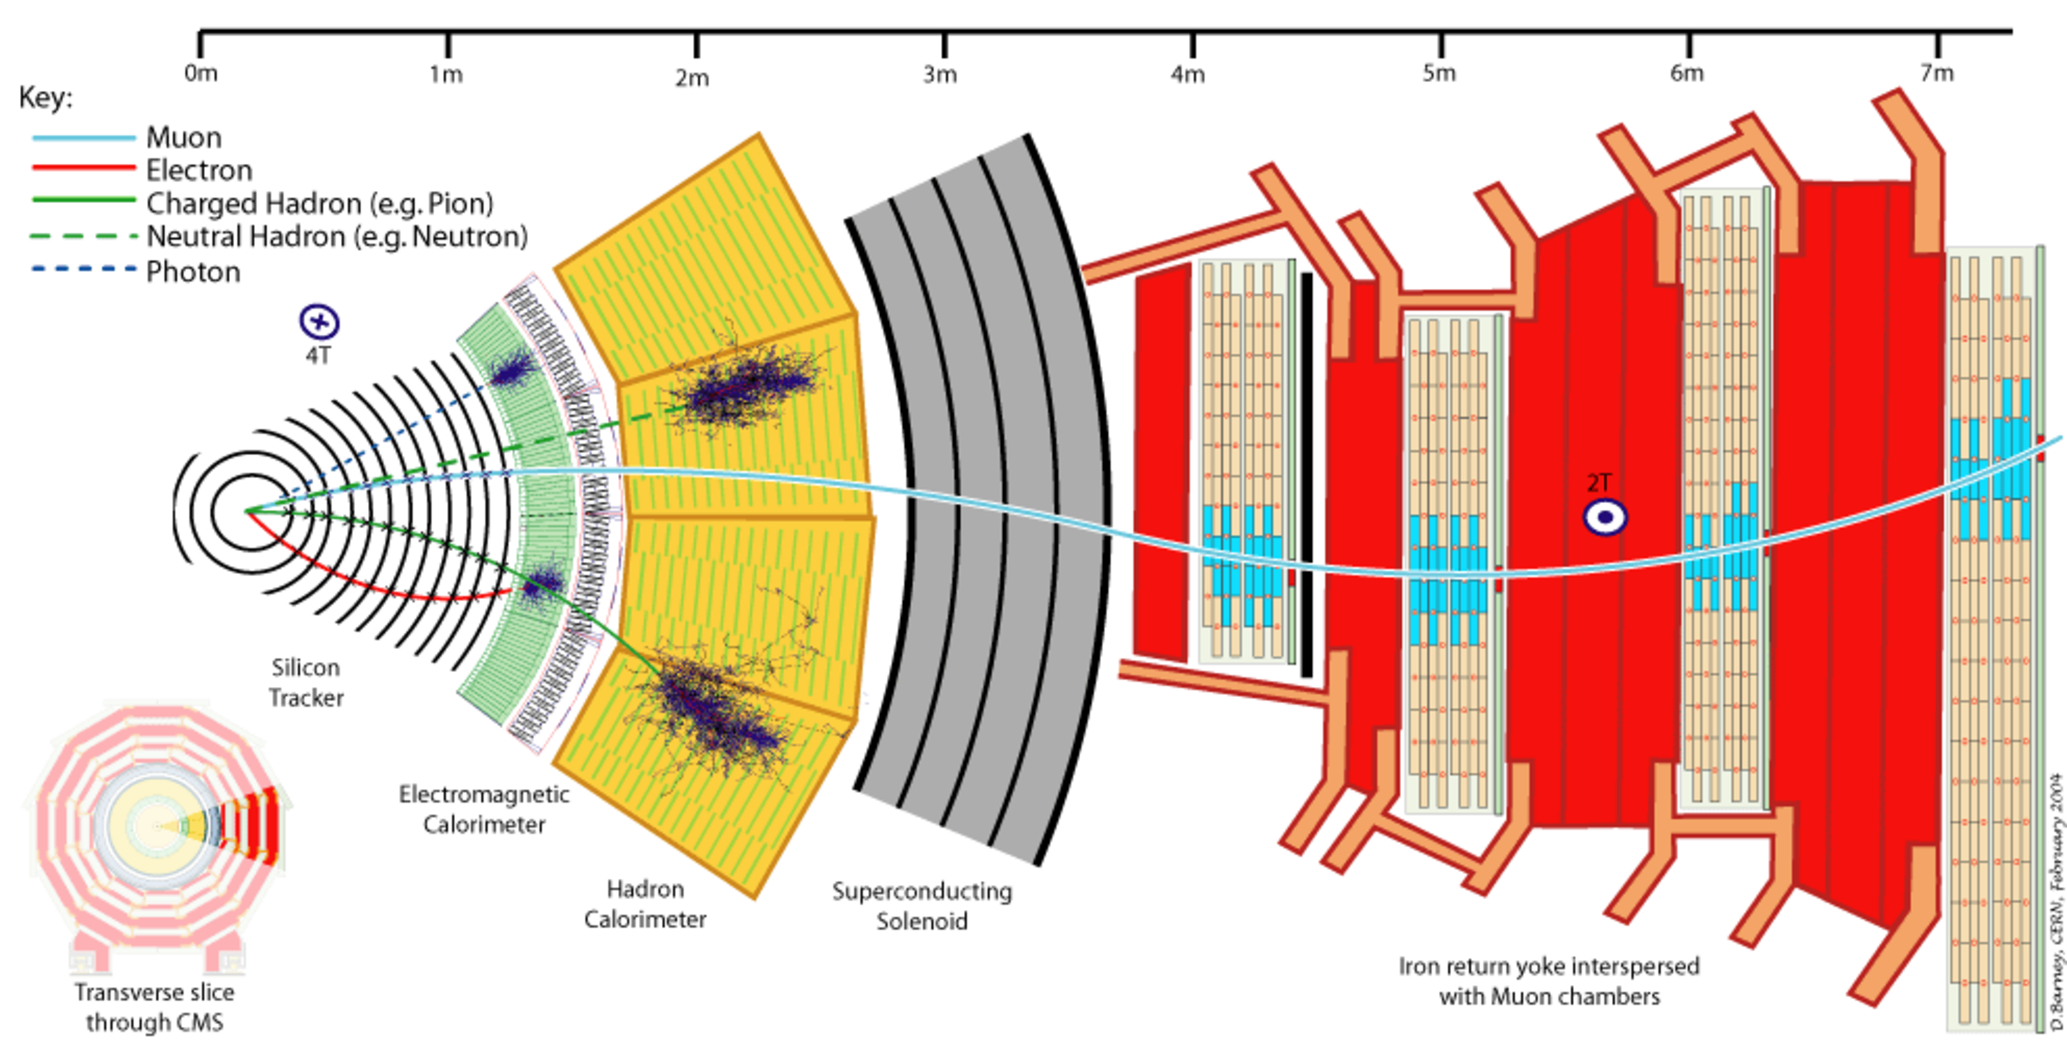
\includegraphics[width=0.8\textwidth]{ch4_figs/cms_particleflow.pdf}
   \caption{An overview of how CMS detects different types of particles. The slice of CMS in in the x-y plane.~\cite{cms_pflow_img}.}
   \label{fig:cms_pflow}
 \end{center}
\end{figure}

Object reconstruction begins with grouping collections of hits into tracks in an iterative process~\cite{CMS-TRK-09-001}. In the first iteration, tracks are
seeded with initial hits and subject to very tight criteria, sacrificing efficiency for a low fake rate. In the following iterations, hits assigned to
tracks in the previous iteration are removed from further consideration, and the criteria for candidate tracks is gradually relaxed with each iteration. In the final iterations,
the constraints on the track seed are relaxed to account for secondary decays from photon conversions and nuclear interactions with the silicon tracker material. This technique
reconstructs tracks with as few as three hits and \pts as small as 150 MeV with a fake rate in the single digits~\cite{CMS-PFT-09-001}. A similar but separate track
reconstruction is performed in the muon chambers to reconstruct muon tracks. 

Object reconstruction continues in the calorimeters, where it relies on a clustering algorithm to identify individual energy deposits and associate them to an object. This
algorithm is designed to yield a high efficiency even for low energy, and nearby objects. The clustering process is performed separately in the ECAL and HCAL, and furthermore in
the barrel, and endcaps. The ECAL preshower also uses separate clusterings in each of its two layers. In the HF, no clustering is performed, where each module is considered an
independent cluster. The clustering algorithm begins by identifying cells (cluster seeds) with an energy above a given ``seed'' energy threshold. Clusters are then increased by
adding adjacent\footnote{sharing at least one edge with the seed} cells that have an energy above a given threshold. The calorimeter granularity is used to optimize the
determination of cluster energies and positions~\cite{CMS-PFT-09-001}.  

After the tracking and clustering is complete, Particle Flow then matches tracks in the tracker to energy clusters in the calorimeters, and to tracks in the muon chambers.
In a given event, there can be many different objects and Particle Flow utilizes
a process-of-elimination strategy. Because they are the easiest to identify unambiguously, muons are identified first by matching tracks in the inner tracker to the tracks in
the muon chambers. The matching criteria is based on a $\chi^{2}$ fit threshold. When multiple sets of tracks are matched, the set with the lowest $\chi^{2}$ is selected as the
muon object. Muons are first reconstructed this way and called global muons~\cite{globalmuon}. Particle flow muons are identifed from global muons when the \pt s measured in the tracker and the
muon chambers agree to within three standard deviations. The tracks corresponding to the muon object are then removed from consideration for the remaining object reconstruction. 

Following muons, electrons are reconstructed next. Because electrons deflect strongly in the magnetic field, they leave characteristically short tracks, and lose energy via
Bremsstrahlung radiation. The tracks are flagged based on these characteristics as potential electron candidates and refitted with a Gaussian-Sum Filter (GSF)~\cite{gsf} and the
resulting tracks are then matched to ECAL energy clusters. The Bremsstrahlung photons are emitted tangentially to electron track and this is accounted for in the ECAL clustering
and track matching specifically for electrons. These matches are then subject to additional quality criteria before they are considered particle flow electrons, and their
corresponding tracks and energy deposits removed from further consideration for the remaining object reconstruction. 

At this point in the event/object reconstruction, the so-called low lying fruit has been picked, and the more difficult objects are all that remain. These objects are charged
and neutral hadrons (jets), and photons. The neutral particles are difficult to reconstruct because they don't leave hits in the tracker, so only calorimeter information is
available. Photons are distinguished from neutral hadrons by separate ECAL and HCAL clusters. Photons interact with and are stopped by the ECAL, while the same is true for
neutral hadrons and the HCAL. Additional in-event calibration techniques are also used to further distinguish these objects. The remainig tracks are subject to tighter
quality cuts aimed at reducing the fake-rate. The high-quality tracks passing these thresholds are matched to ECAL and HCAL deposits, and give rise to particle flow 
charge hadrons. The momentum of these objects is measured from the track radius and compared to the corresponding energy deposit in the calorimeters assuming the object is
a charged pion. If the two measurements are compatible, the momenta is refined with additonal fits to the tracks and energy deposit(s)~\cite{CMS-PFT-09-001}.

The charged and neutral hadron objects with tracks and matched energy deposits are only considered particle flow candidates at this stage.
An additional clustering step is necessary to reconstruct jet objects. As mentioned previously, when free quarks produced in the pp collision decay in the
fragmentation/hadronization process, they produce energetic and collimated sprays of charged
and neutral hadrons, called jets. To accurately determine the direction and momentum of the initial quark, as many of the corresponding charged and neutral hadrons as possible must not only be
reconstructed correctly and identified, but also clustered together (matched) correctly.
These jets are then intrepreted experimentally to be the free quark. An depiction of the hadronization and jet detection process is below in Figure~\ref{fig:frag}.

\begin{figure}[hbtp]
 \begin{center}
   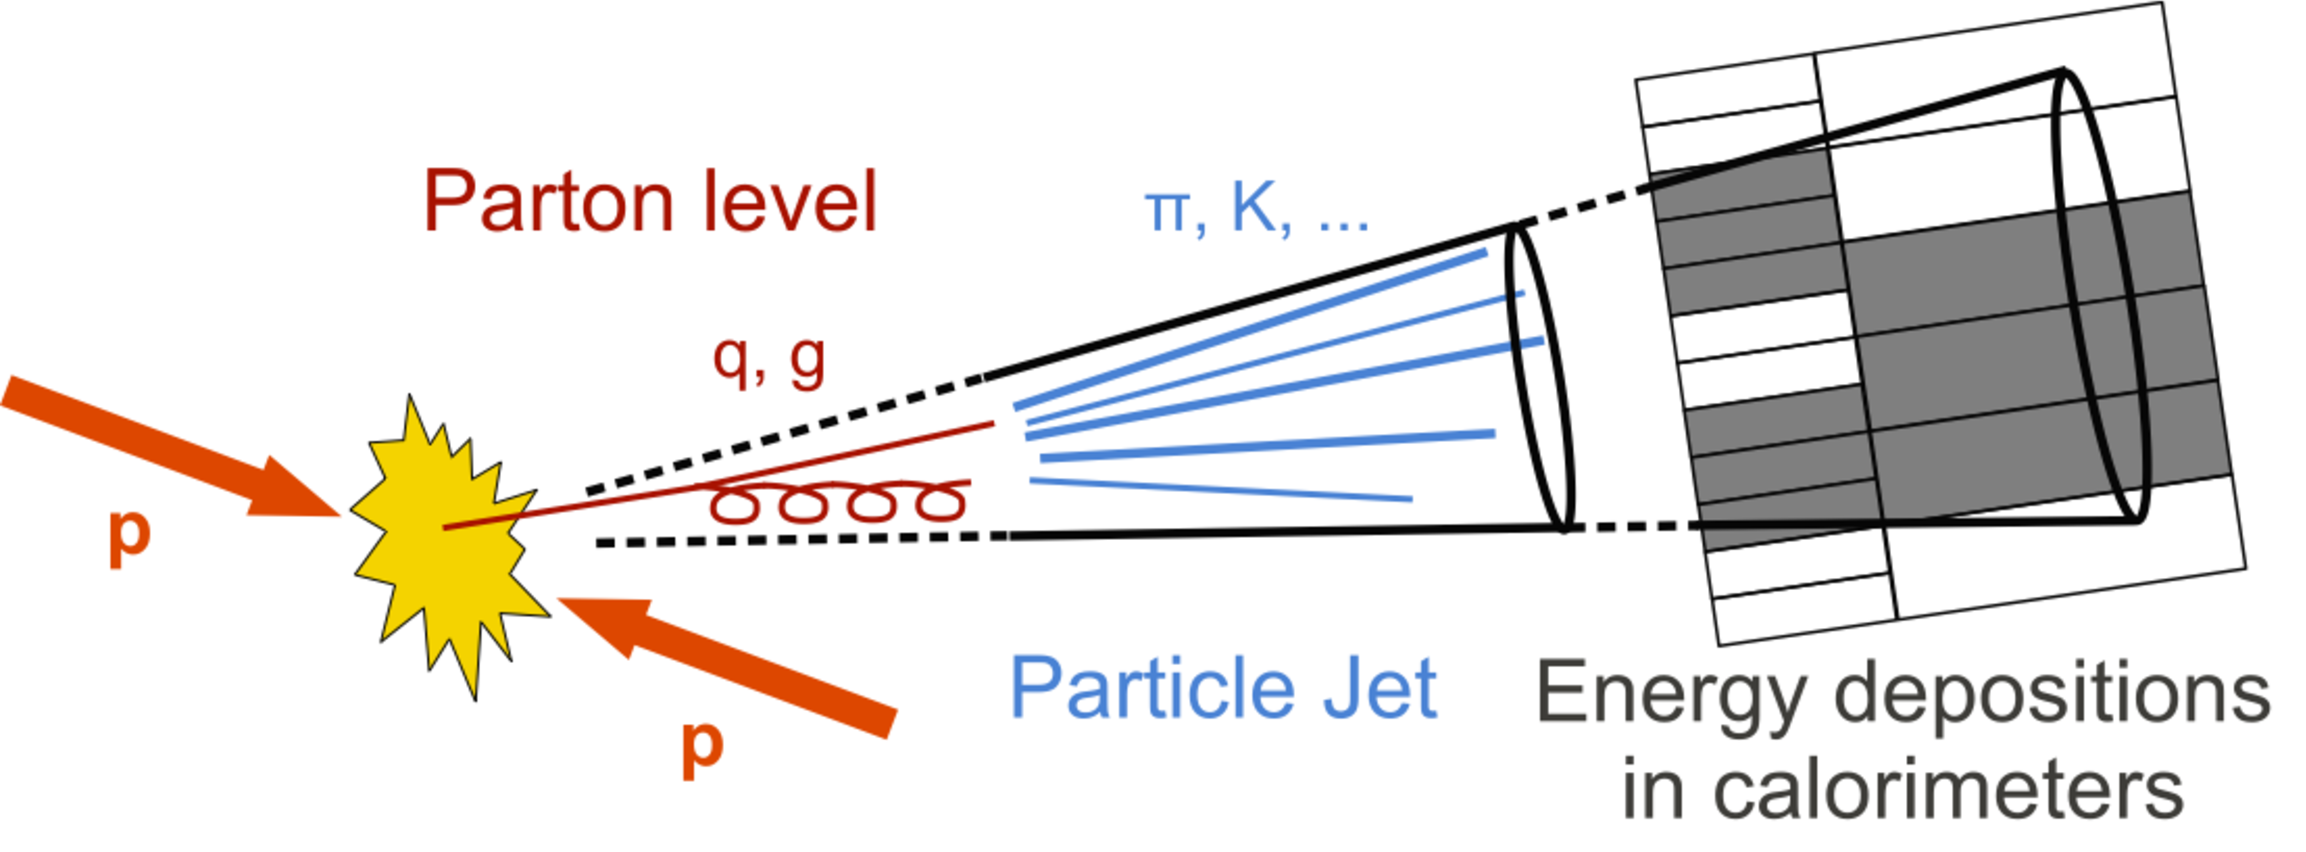
\includegraphics[width=0.8\textwidth]{ch4_figs/jet_frag.pdf}
   \caption{An example of quark hadronization and the resulting jet.~\cite{frag}.}
   \label{fig:frag}
 \end{center}
\end{figure}
 
There are too many PF candidates detected and reconstructed in the calorimeters in a given event at one time to make the jet clustering process straight-forward
and unambiguous. To address this, jet clustering algorithms are used for clustering. These algorithms exploit information from the detector with theoretical knowledge of the
hadronization process to cluster the jets sensible and reproducible manner.
While many clustering algorithms exist, the one used by this analysis is the anti-$k_{T}$ algorithm~\cite{antikt}. Anti-$k_{T}$ begins like other sequential clustering algorithms,
by calculating the distance measures in equations~\ref{eqn:antikt1}. 

\begin{equation}
\begin{aligned}
\label{eqn:antikt1}
%%\begin{split}
d_{ij} &= min(k^{2p}_{Ti},k^{2p}_{Tj})\frac{\Delta_{ij}^{2}}{R^{2}} \\ d_{iB} &= k^{2p}_{Ti}
%%\end{split}  
\end{aligned} 
\end{equation}

\noindent where $\Delta_{ij}^{2} = (y_{i}-y_{j})^{2} + (\phi_{i}-\phi_{j})^{2}$ and $y_{i}$,$k_{Ti}$ are the rapidity and momenta of particle i respectively. After the
distance measures have been calculated for each candidate in the event, the smallest $d_{ij}$ are merged into one object by summing the 4-momenta of particles i and j, the
distance measures are updated and the algorithm moves onto the next smallest $d_{ij}$. If a particle has the smallest $d_{iB}$, it is removed and called a jet. This
iterative process continues until all PF candidates are clustered into jets. What differentiates anti-$k_{T}$ from Cambridge-Aachen and other similar algoirthms is the choice
of p = -1 in equation~\ref{eqn:antikt1}. This negative value explains the name of the algorithm, and the tendancy for it to produce circular\footnote{circular in the
$\eta$-$\phi$ plane} jets, centered on the highest \pt~candidate of the jet. The effect of these parameter values with respect to other available algorithms is below in
Figure~\ref{fig:jet_cluster}.

\begin{figure}[htbp] 
  {\centering
    \subfigure[$k_{T}$]{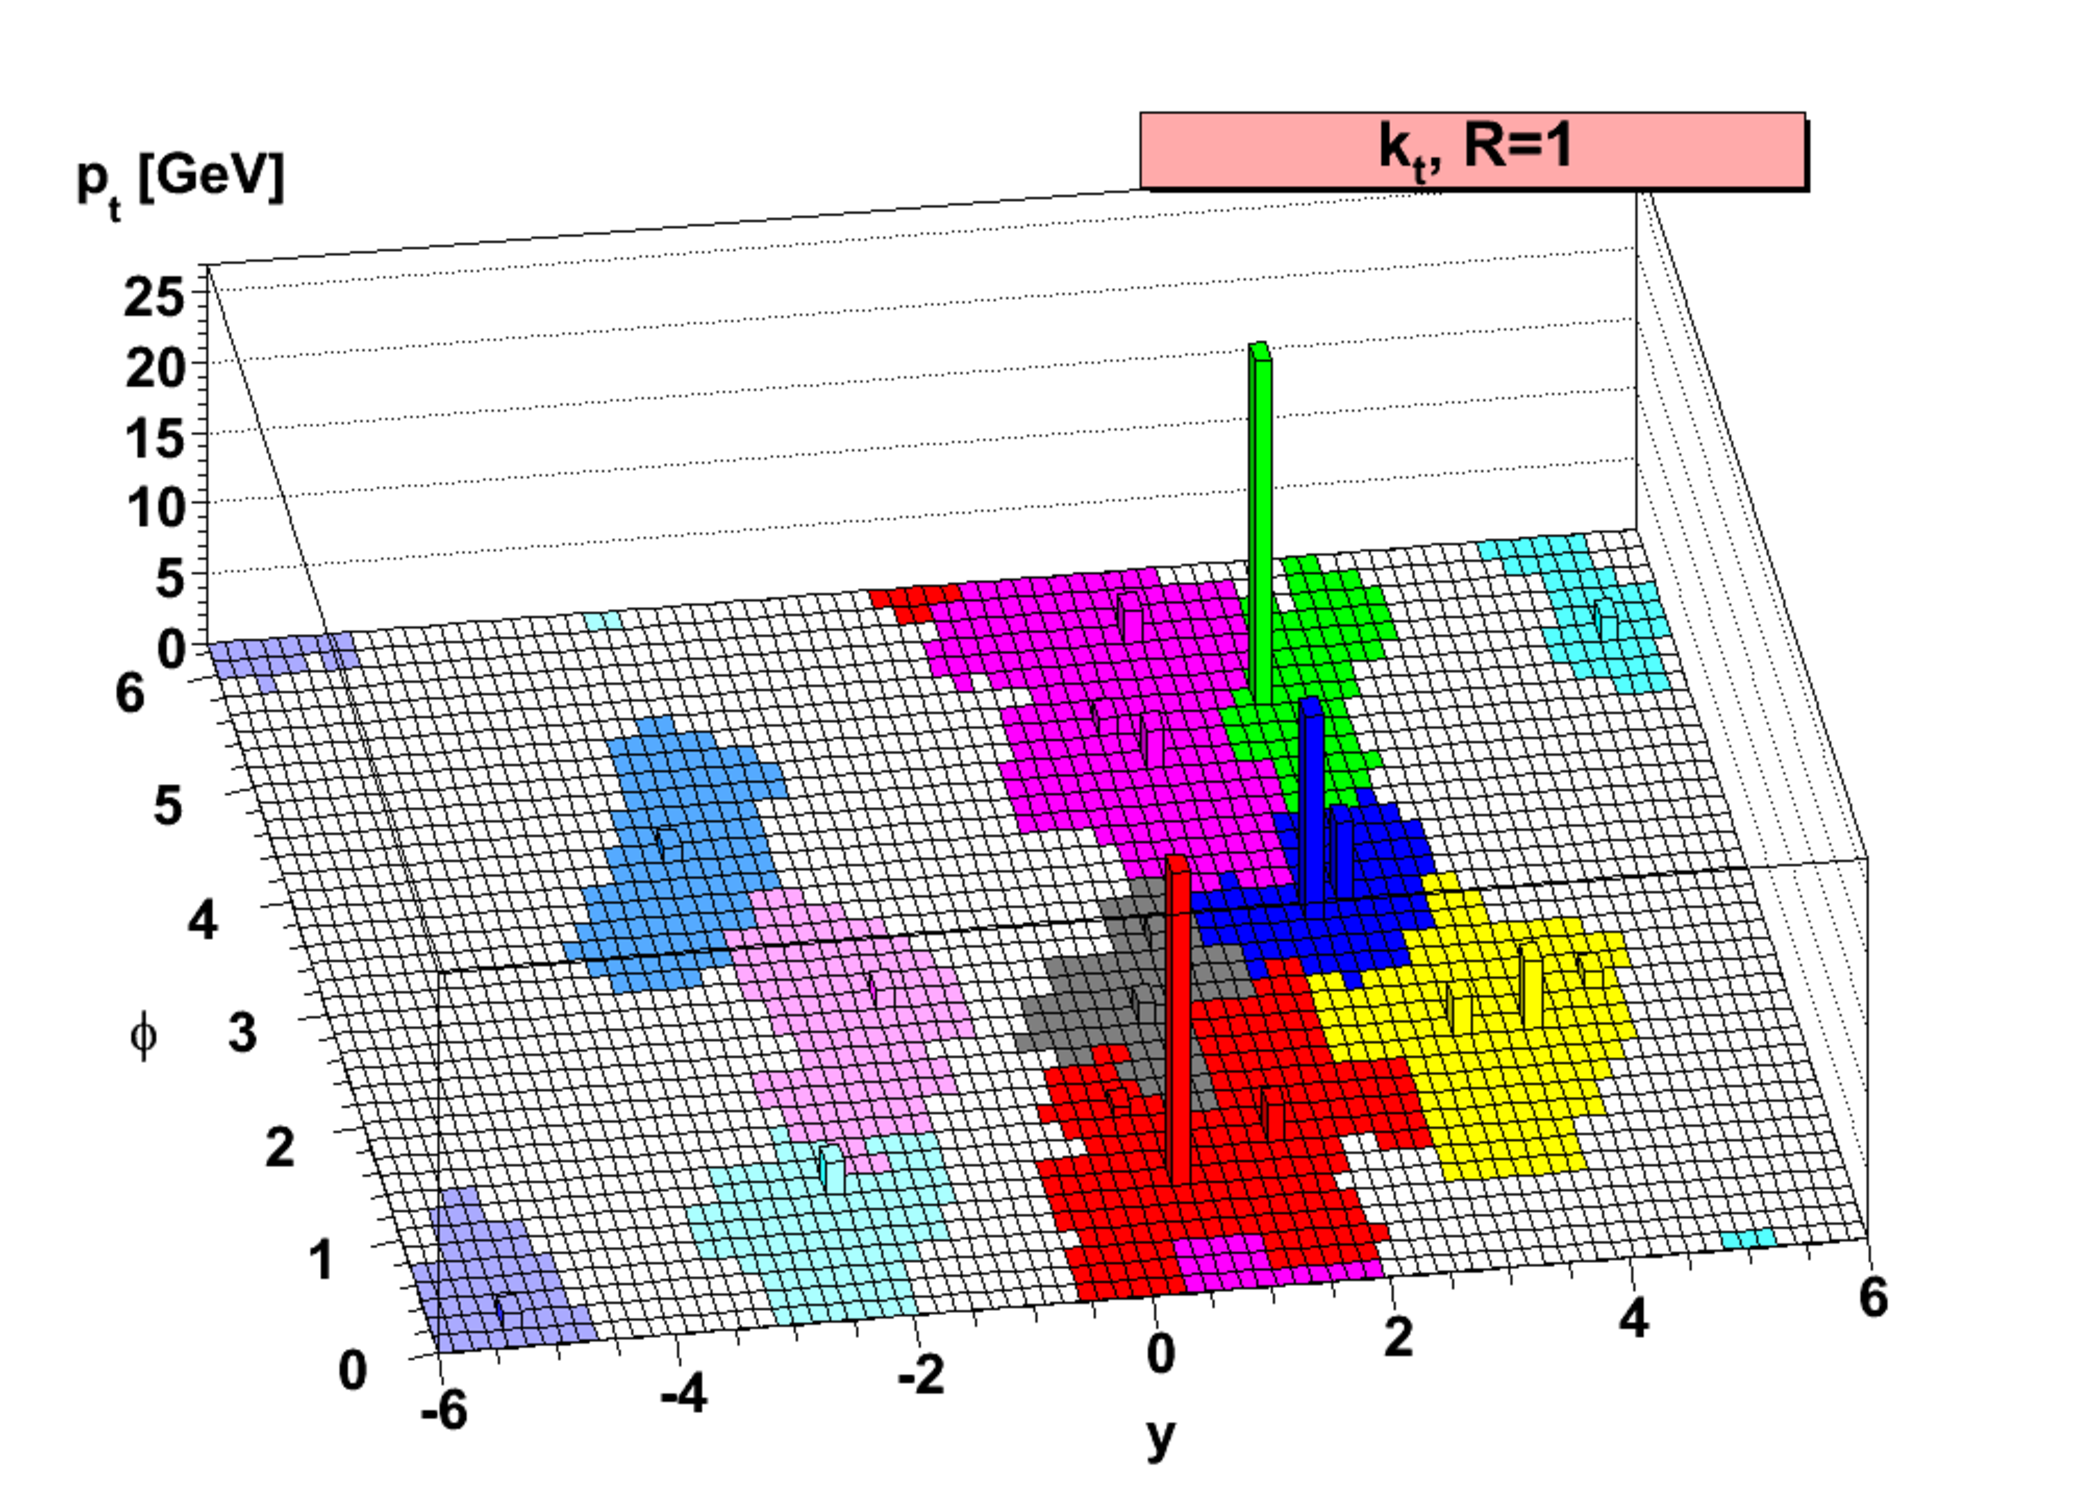
\includegraphics[width=0.4\textwidth]{ch4_figs/kt.pdf}}
    \subfigure[Cambridge-Aachen]{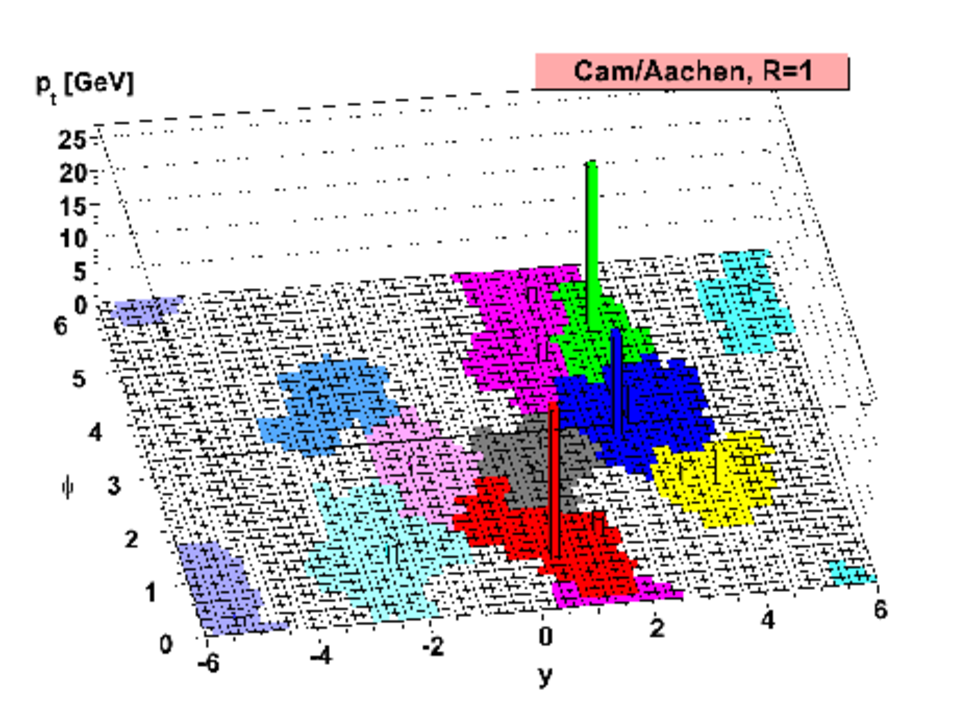
\includegraphics[width=0.4\textwidth]{ch4_figs/ca.pdf}}
    \subfigure[SIScone]{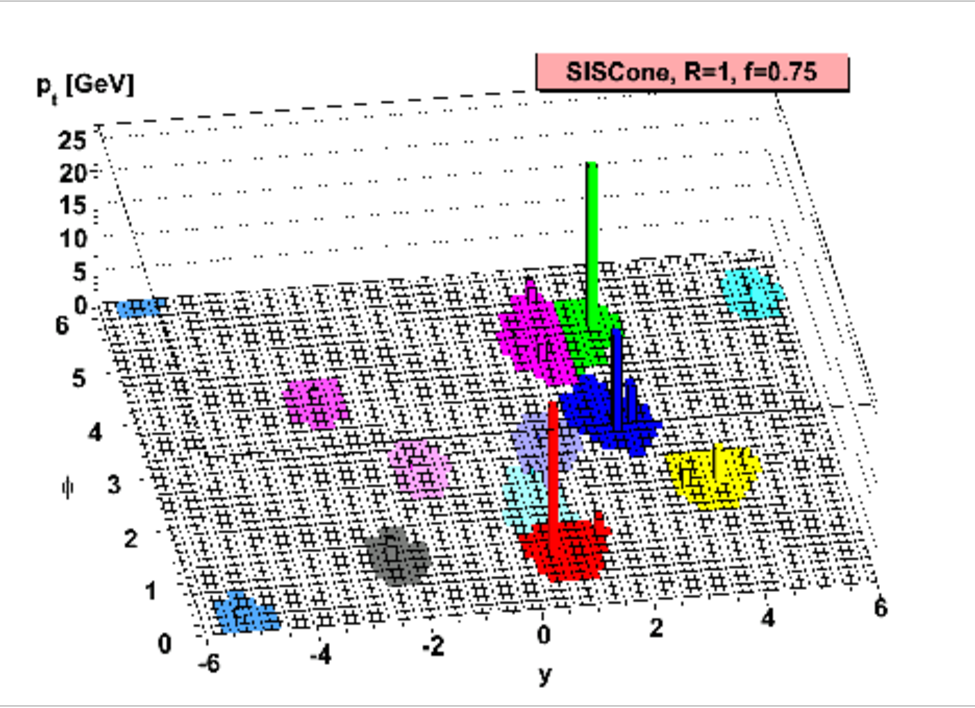
\includegraphics[width=0.4\textwidth]{ch4_figs/sis.pdf}}
    \subfigure[anti-$k_{T}$]{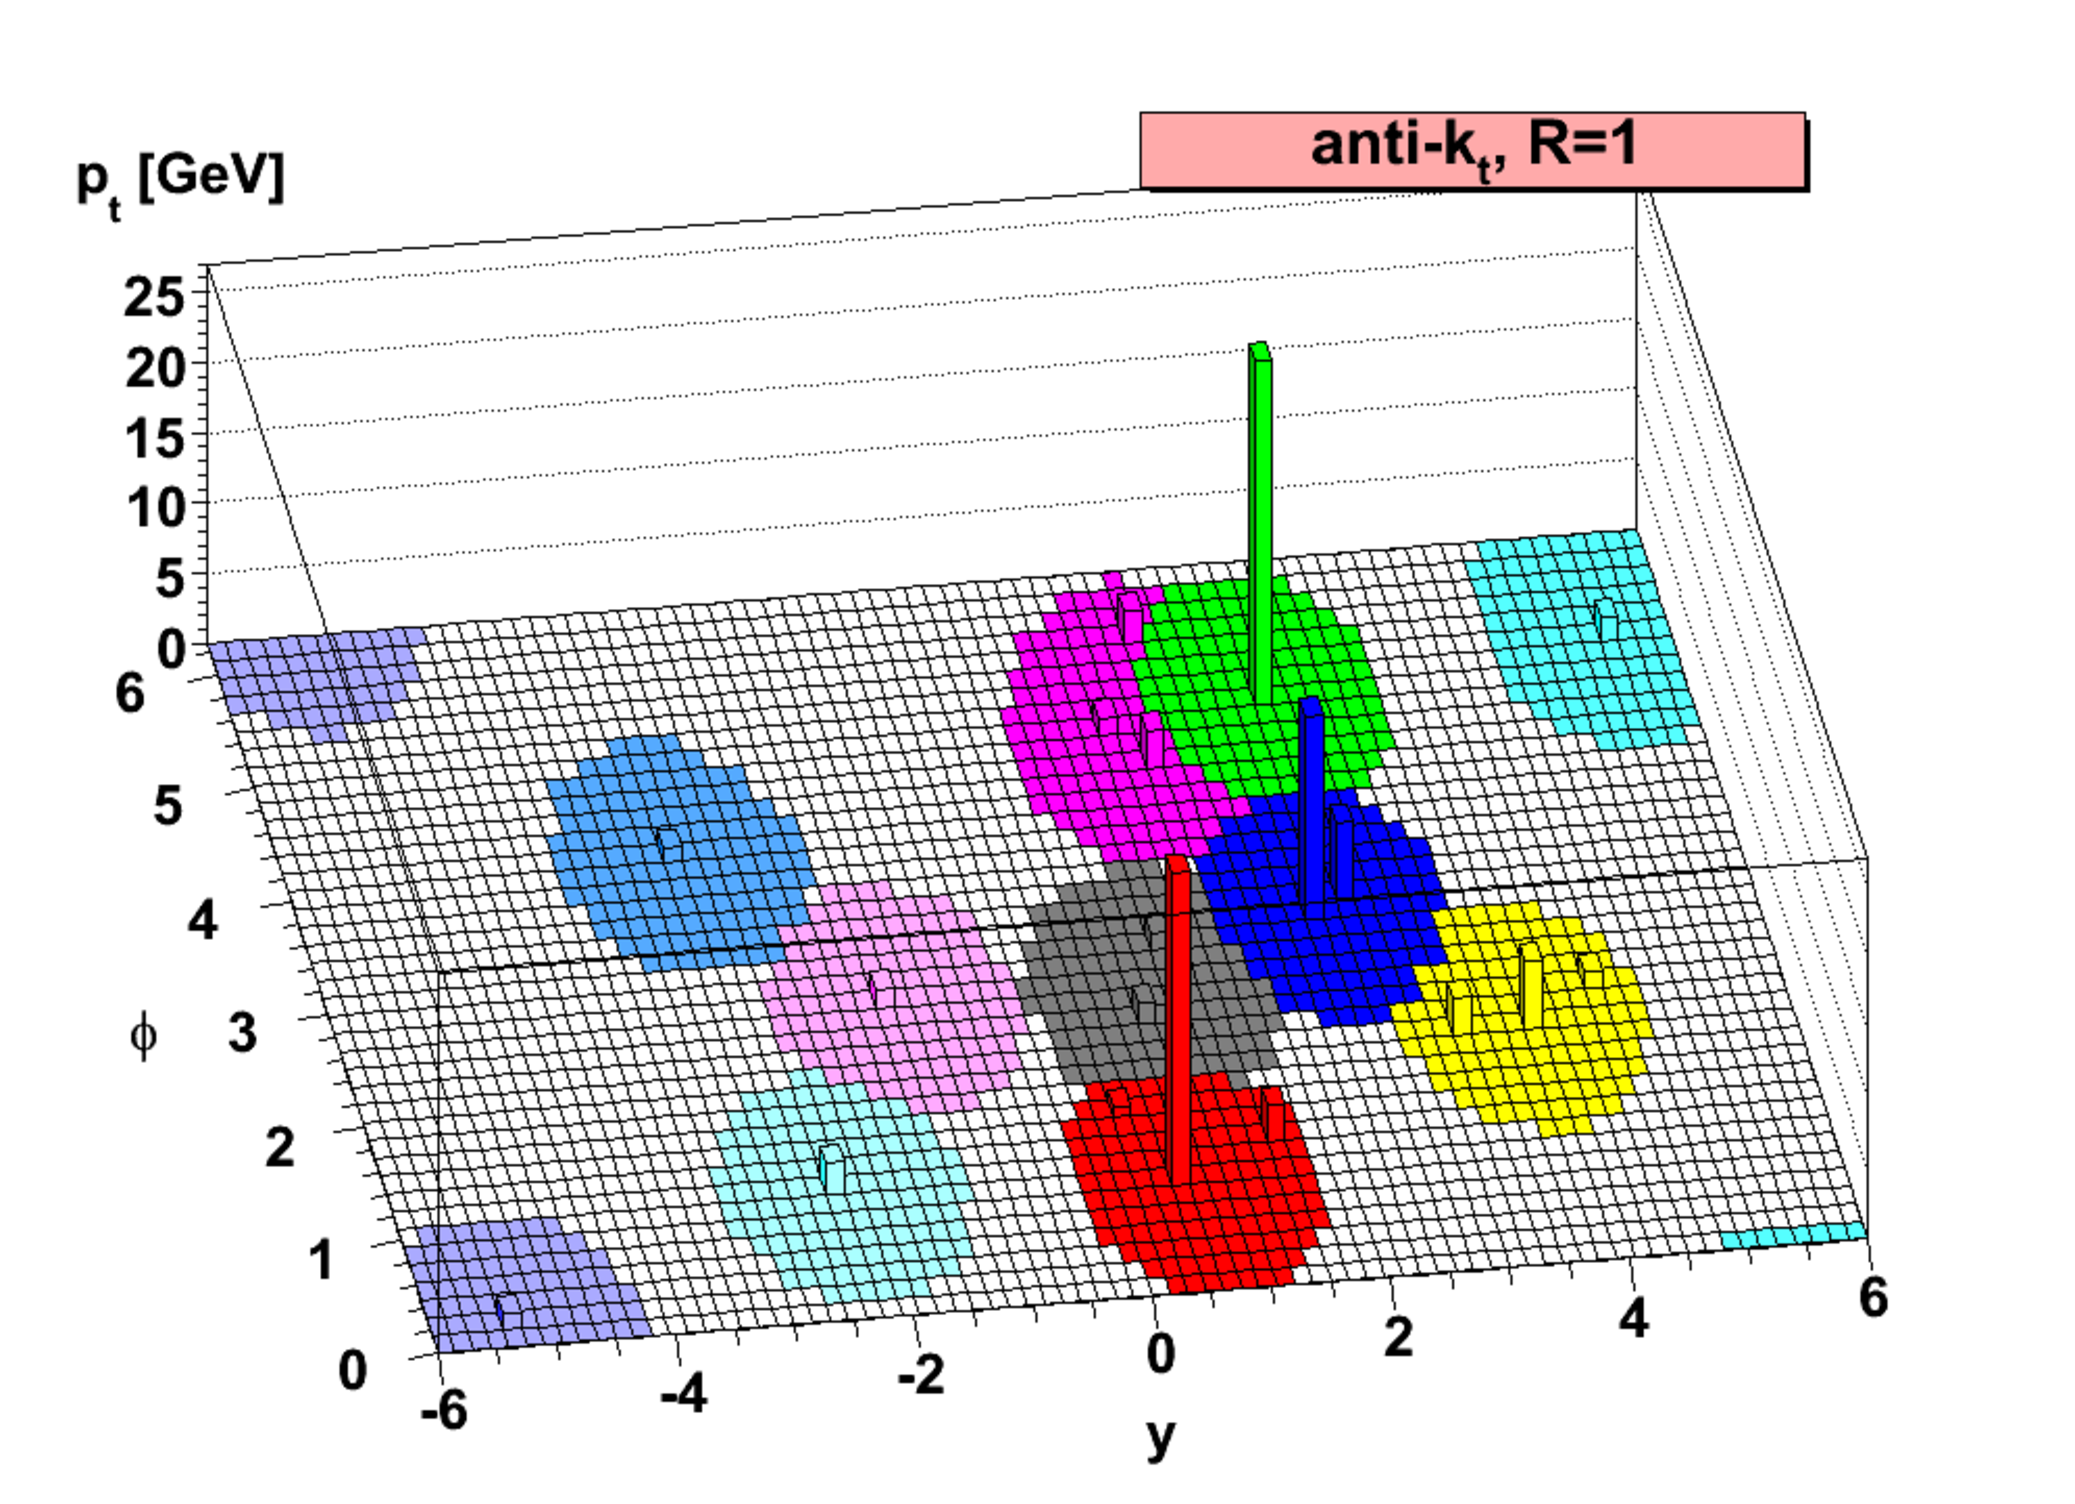
\includegraphics[width=0.4\textwidth]{ch4_figs/akt.pdf}}
    \caption{Jets in a sample MC event clustered with various algorithms.
    \label{fig:jet_cluster}}
\end{figure}

The final parameter in equation~\ref{eqn:antikt1} is defined as $R = \sqrt{\Delta\eta^{2}+\Delta\phi^{2}}$ is the conesize of the jet being clustered.
The cone size used for clustering in this analysis is R = 0.4. Versions of this analysis on 7, and 8 TeV datasets used a wider cone of 0.5. The move to smaller cone size
was motivated by the fact that jets tend to be more energetic and thus narrower and more collimated as the center-of-mass collision energy increases to 13 TeV. All techniques
mentioned above proved CMS analyzers the basic physics objects needed to perform analysis, and also standardizes the object reconstruction across the experiment. 

\section{Primary Vertex Identification and Pile-up}
Due to the way the LHC collides bunches, there are multiple pp collisions in each LHC bunch crossing at CMS. Unfortunately, many of these collisions produce
multiple objects that are reconstructed, but only 1 of these collisions is considered a hard scatter head-on collision capable of producing a \tth event.
These additional collisions that don't include the hard scatter event of interest, as well as their resulting reconstructed objects are referred to as pile-up, because
they are said to pile up on top of the objects from the collision of interest.
The collision of interest is called the primary vertex.
In this analysis and also in many others, the primary vertex is defined as the vertex with the highest \pt~sum of all constituent tracks.  
Pileup is problematic because it can make matching objects to collisions difficult. Fortunately,
CMS has an excellent tracker which makes the process of matching tracks to vertices (collision) fairly straightforward. Aside from the tracking, pileup is also
problematic because the energy deposits in the calorimeters from the pilup objects can distort the energy measurements and clustering of objects originating from
the primary vertex. There are numerous techniques to account for these effects. The technique employed in this analysis is to assign an average amount of energy
due to pileup in the detector, and subtract it off from each reconstructed jet energy measurement. This is called the rho correction.  
An example of the reconstructed tracks and vertices in an
LHC bunch crossing is below in Figure~\ref{fig:pileup_vertices}.

\begin{figure}[hbtp]
 \begin{center}
   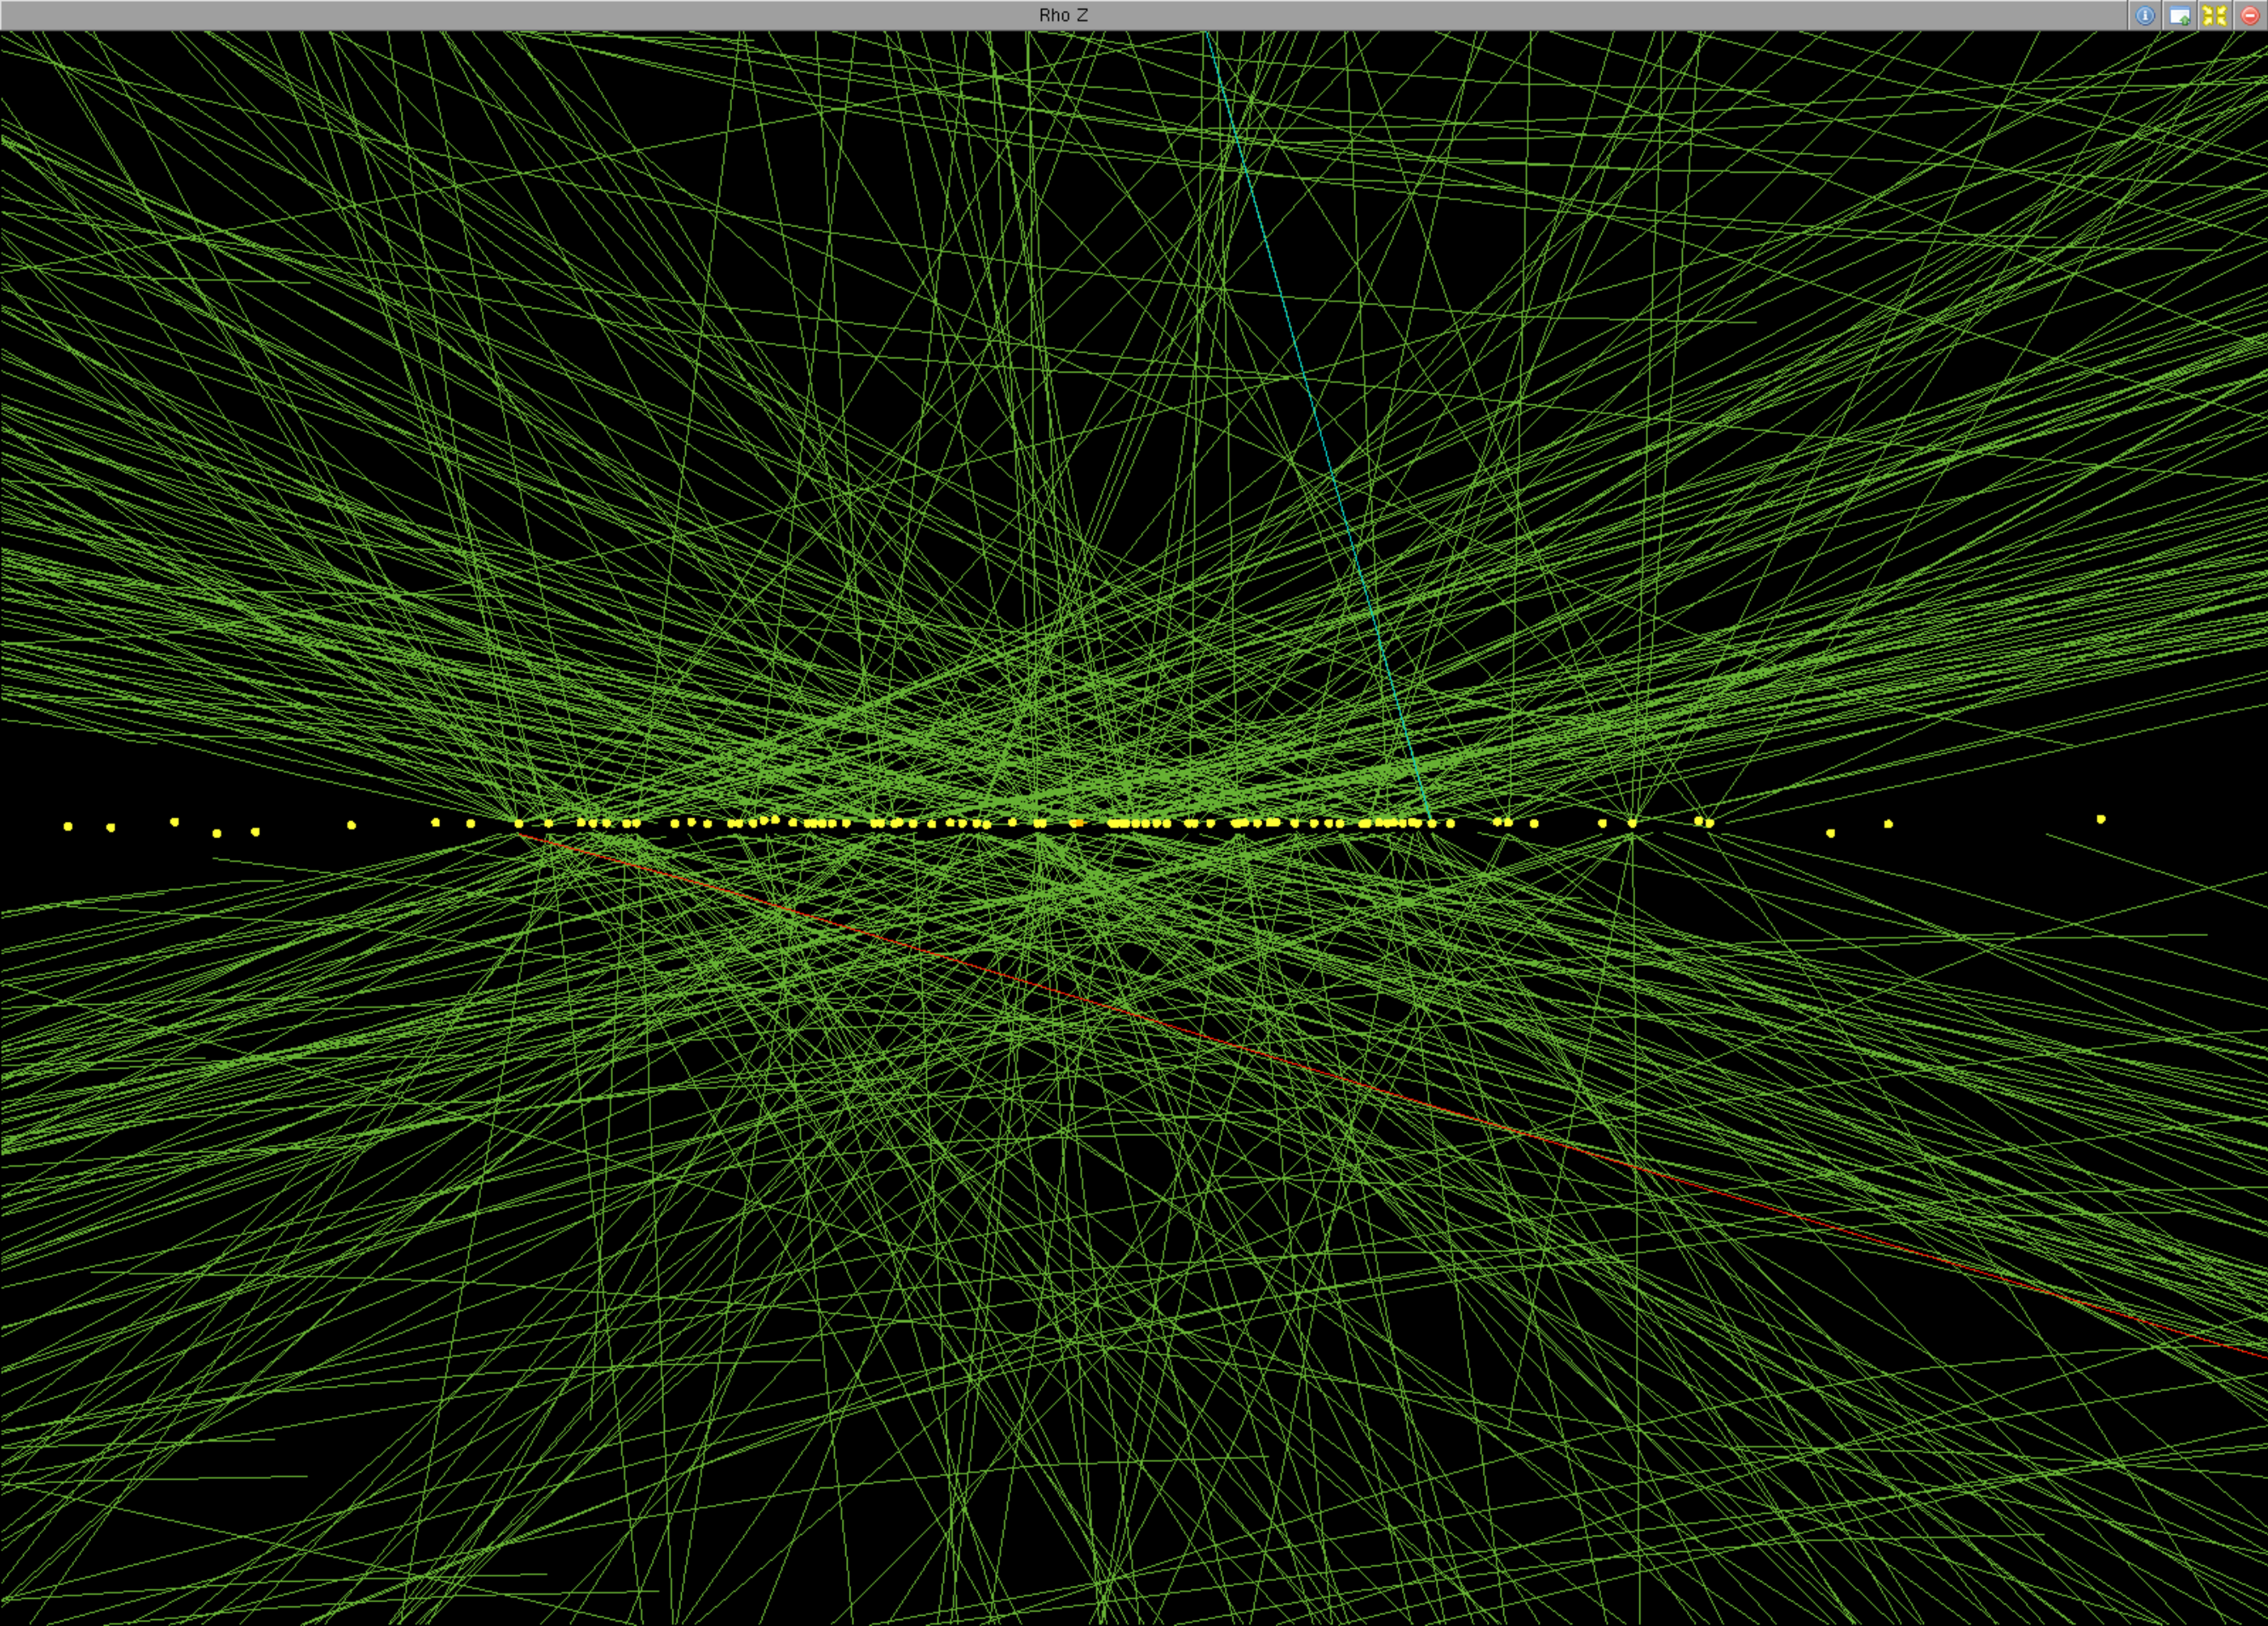
\includegraphics[width=0.8\textwidth]{ch4_figs/cms_pileup.pdf}
   \caption{A side view of the CMS tracker's reconstructed vertices in a special high pileup LHC run. The pileup in this here is 78, meaning there are
78 collisons in a single bunch crossing~\cite{pileup_image}.}
   \label{fig:pileup_vertices}
 \end{center}
\end{figure}

\noindent The pileup values in the data in this analysis varies from 30 to 45, meaning there are, on average, between 30 and 45 collisions (including the primary vertex) in each
bunch crossing recorded by CMS. 

\section{Object Selection}
After the basic object reconstruction is performed, each event is ready for the fist steps of analysis. The analysis begins with object selection where the objects in each
event are subjected to tighter criteria to ensure quality objects in the analysis that are consistent with signal and background predictions. This selection depends on and 
varies with the type of object desired in the event. Because the \tth multilepton final state is so complicated, almost\footnote{all objects except the photon, which are
used in the \tth,$H\rightarrow\gamma\gamma$ search} all objects available from the particle flow
reconstruction are needed to identify events that are consistent with the signal, namely jets, missing energy, charged leptons, and hadronic taus.

\subsection{Jets}
Jets are clustered with anti-kt and reconstructed from PF candidates as described previously using the FASTJET algorithm~\cite{antikt}\cite{fastjet}.
Charged hadrons not originating from the primary vertex are subtracted from the jet clustering. Because the detector performance varies with time the measured jet energies
must be updated to correct for performance degradation in the calorimeters. The jets are corrected in bins of jet $E_{T}$ (transverse energy) and $\eta$~\cite{jec}.

The jet selection for this analysis requires jets to have a \pt $>$ 25 GeV and $|\eta|$ $<$ 2.4. Jets are removed when they overlap with a fakeable lepton (described later) within
a $\Delta$R cone of $<$ 0.4. Finally, the jets must pass the working point of the an MVA used to discriminate against jets from pileup vertices. This discriminator uses inputs
characterizing the shape of the jet, the relative amounts of charged and neutral candidates within the jet, and the \pt ratio between the candidates. 

\subsection{b-jet Identification}
The properties of heavy flavor quarks, specifically the bottom quark, have unique characteristics that make their hadronizations easy to identify or tag. This identification is called
b-tagging and used throughout this and many other analyses. These heavy flavor quarks are characterized by large\footnote{large relative to light quarks and gluons} masses,
long lifetimes, high \pt decay products among which there is an occasional charged lepton. The long lifetime provides a key handle to identify b-decays, since the b travels farther before
decay and producing a secondary vertex. Identifying this secondary vertex plays a central role in tagging jets from b-decays. All of properties are measured by CMS and used to discriminate b-quark jets
from light flavor QCD jets. 

Jets originating from b-quark hadronization (b-jets). Identifying b-jets is crucial to selecting \tth events since the tops
almost always produce b-quarks. The algorithm used in this analysis is the Combined Secondary Vertex (CSVv2) tagger~\cite{csvv2}. The CSVv2 tagger is an MVA discriminator that
combines secondary vertex information with impact parameter variables that discriminate heavy flavor quarks from light flavor quarks and gluons. The tagging variable is assigned
for each jet, and can range from -1 to +1, where the higher values correspond to higher likelihood that the jet originated from a b-quark. The jets described in the previous
subsection are \emph{tagged} when they pass a specific working point of the tagger. The specific working point is choosen to balance keeping the fake rate low, and the efficiency
high. The working points used in this analysis were selected after studying the tagger performance, as a function of jet \pt and $\eta$ in data samples with b-jets. Two working points
are used for b-tagging in this analysis. The medium working point (CSVv2 $>$ 0.8484) corresponds to 70\% efficiency for tagging
b-jets with a 1.5\% mistag rate, while the loose working point (CSVv2 $>$ 0.5426) corresponds to an 85\% efficiency and a 10\% mistag rate. The mistag rate is the rate is the efficiency
to tag jets with only light flavor quarks or gluons. The motivation for two working points is explained in the event selection. 

\subsubsection{b-jet Scale Factors}
The shape of the CSVv2 distribution of b-jets in data differs somewhat between that of MC. Because MC is being used to predict both the signal and many of the backgrounds, we apply scale factors (SFs)
to correct the shape in the MC to match that of data. These scale factors are derived separately for heavy (b,c quark) flavor and light flavor as a function of the jet CSVv2, \pt, $|\eta|$. The SF is 
calculated according to equation~\ref{eqn:csvsf} below. 

\begin{equation}
\label{eqn:csvsf}
  SF(CSVv2,p_{T},\eta) = \frac{DATA-MC_{A}}{MC_{B}}
\end{equation}

\noindent where A/B = light/heavy flavor for the heavy flavor correction and A/B = heavy/light for the light flavor correction. The scale factors are derived from a tag-and-probe technique. First,
a control region is defined by selecting opposite sign $e-\mu$ events with exactly two jets. When this selection is applied to data, it yields events enriched with di-leptonic \ttbar decays where the
two jets are most likely b-jets. Then one of the jets (the \emph{tag}) is required to pass the medium CSVv2 working point (CSVv2 $>$ 0.8484) to increase the \ttbar purity. In real \ttbar events, the
remaining jet (the \emph{probe}) is very likely a b-jet. Because control region applied to data is only \emph{enriched} in \ttbar events and not pure \ttbar events, we subtract off the contribution of
light flavor jets as estimated in MC, which explains the second term in the numerator of equation~\ref{eqn:csvsf}. Now we can directly apply this same control region to pure \ttbar MC, and the ratio
of the corrected yields in data to the pure \ttbar MC gives the scale factor described in equation~\ref{eqn:csvsf}. The same process is used for the light flavor correction, but the control region
definition is modified to instead select dileptonic events with two leptons that have the same flavor and opposite sign, with exactly two jets where one of the jets \emph{fails} the medium CSVv2 WP.
This control region applied on data yields events enriched in Z+jets and the tag-and-probe process is repeated. The full details of this technique are described in~\cite{CMS-AN-2013-130}~and~\cite{csvsf_twiki}.

\subsection{Missing Energy}
Missing energy, or more accuarately missing \emph{transverse} energy is calculated as the negative vector sum of \pt of all PF candidates in the event, denoted as \met. It is called missing because
the gluons (or quarks) colliding in the hard scatter that produce events such as \tth have no initial transverse momentum. By momentum conservation, the vector sum of all particles
produced in the collision should match the sum before the collison. Any time the \met is non-zero, it is assumed to be carried off by missing particles. In the context of this and many other analyses,
the \met is interpreted as the presence of neutrinos. The two same-sign lepton requirement on the signal ensures that there will always be two neutrinos in the event, making it impossible to fully
reconstruct the individual neutrino momenta. The presence of \met can also arise due to mis measurements, incorrect reconstructions or jet clusterings, or the contribution of pile up events. To discriminate
between the different sources of \met we use another variable called \HT, which is the negative vector sum of all selected jets and leptons in the event. While \HT has lower resolution than the \met,
it relies only on the higher \pt selected objects and not the softer objects failing the seleciton. To exploit the fact that \HT and \met are less correlated in events with incidental missing energy,
and more correlatd in events with real missing energy, a linear discriminat of both varibles is used and defined as

\begin{equation}
\label{eqn:metld}
 \met LD = \met\times0.00397 + \HT\times0.00265
\end{equation}

\noindent where the \met LD value is cut on which will be described in the event selection. 

\subsection{Leptons}
The flagship objects that characterize this analysis are the leptons. The lepton selection is the foundation of this \tth search and many of the analysis treatment that follows later is due to the
choice of lepton selection. The ultimate goal of the lepton selection is to identify and select prompt leptons and reject non-prompt, also known as fake, leptons. In this context, a prompt lepton
is a lepton that originates directly (promptly) from a W, Z or $\tau$\footnote{prompt leptons produced in $\tau$ decays are actually coming from an offshell W produced by the decaying $\tau$} decay, while non-prompt leptons
predominantly originate from b-hadron decays, but also in-flight decays of pions, and photon conversions. The term \emph{fake} is used to describe non-prompt leptons because non-prompt leptons
that pass the criteria designed to select prompt leptons are faking prompt leptons. These fakes are one of the largest backgrounds in this analysis and the lepton selection is designed to reduce both
the quantity of fakes entering the signal regions, and the systematic uncertainties on that quantity. 

\subsubsection{Electron Identification}
Electrons are reconstructed from tracker hits (GSF tracks) and ECAL clusters via particle flow as described previously. While many other criteria is placed on electrons later, they first must
have $|\eta|<$2.5 to be guarantee they passed through the tracker, and minimum \pt $>$ 7 GeV. Electrons must pass the working point of an MVA designed to identify electrons using shower-shape variables,
track-cluster consistency variables, and track quality variables~\cite{elemvaid}. We apply loose cuts as a function of $|\eta|$ on this MVA value. The full shape of this MVA is used as an input to
the Lepton MVA, which will be described in the following sections. 

\subsubsection{Muon Identification}
Muons are reconstructed by combining tracks from the silicon tracker with tracks in the muon chambers and are required to be global muons. Muons are first required to have \pt $>$ 5 GeV and
$|\eta|<$2.4. We use centralized selectrion criteria developed by the CMS
Muon Physics Object Group (POG) and require all muons to pass the Loose ID~\cite{loosemuon} and in some cases the Medium ID~\cite{mediummuon} depending on the selection. 

\subsubsection{Isolation}
Lepton isolation is a measure of how spatially isolated the lepton is from other physics objects in the detector in an event. Prompts leptons are typically isolated from hadronic activity
(jets) in the event, while non-prompt leptons, which are often produced in hadronic decays, are significanly less isolated and close to/overlapping with jets. The standard isolation considers
all charged and neutral hadrons as well as photons within a fixed cone size in R around the lepton, then if there is too much energy relative to the lepton energy from the
other objects inside the fixed cone radius, the lepton fails the isolation criteria. This analysis uses a variation of this technique that varies the cone size with the \pt of the lepton, since
boosted (very high momentum) objects tend to be more collimated and thus should have a more collimated cone definition. This isolation technique is called mini isolation (\miniIso) and the cone
size is varied with lepton \pt according to equation~\ref{eqn:miniIsoConeSize} below. 

\begin{equation}
\label{eqn:miniIsoConeSize}
 R = \frac{10}{min(max(p_{T}(l),50),200)}
\end{equation}

\noindent The amount of activity inside this cone is adjusted to correct for pileup using the $\rho$-correction, which assumes a fixed pileup-density in different $|\eta|$ ranges in the detector. The
pileup density $\rho$, is multiplied by effective areas as a function of $|\eta|$. The \miniIso quantity is defined in equation~\ref{eqn:miniIso} below

\begin{equation}
\label{eqn:miniIso}
 I_{mini} = \frac{\sum_{R}p_{T}(h^{\pm}) - max(0,\sum_{R}p_{T}(h^{0}) + p_{T}(\gamma) - \rho A (\frac{R}{0.3})^{2}) }{p_{T}(l)}
\end{equation}

\noindent where $\sum_{R}p_{T}(h^{\pm})$ is the energy of the charged hadrons inside the cone of radius R, $\sum_{R}p_{T}(h^{0})$ is the energy of the neutral hadrons inside the cone, $p_{T}(\gamma)$ is
the energy from photons inside the cone, and $-\rho A (\frac{R}{0.3})^{2}$ is the correction for pileup. The effective areas, A, are defined separately for muons and electrons and are based off a fixed
cone size of R = 0.3 and listed in tables~\ref{tab:ele_effArea}\ref{tab:mu_effArea}, which explains the denominator in the pileup correction term. Both muons and electrons are subject to the same isolation criteria, which requires \miniIso $<$ 0.4.

\begin{table}[hbtp]
\centering
\caption{Electron effective areas for the pileup correction.}
\begin{tabular}{lcc}
\hline
$|\eta|$ range & effective area \\
\hline
$|\eta| < 1.0$ & 0.1752 \\
$1.0 < |\eta| < 1.479$ & 0.1862 \\
$1.479 < |\eta| < 2.0$ & 0.1411 \\
$2.0 < |\eta| < 2.2$ & 0.1534 \\
$2.2 < |\eta| < 2.3$ & 0.1903 \\
$2.3 < |\eta| < 2.4$ & 0.2243 \\
$2.4 < |\eta|$ & 0.2687 \\
\hline
\end{tabular}
\label{tab:ele_effArea}
\end{table}

\begin{table}[hbtp]
\centering
\caption{Muon effective areas for the pileup correction.}
\begin{tabular}{lcc}
\hline
$|\eta|$ range & effective area \\
\hline
$|\eta| < 0.8$ & 0.0735 \\
$0.8 < |\eta| < 1.3$ & 0.0619 \\
$1.3 < |\eta| < 2.0$ & 0.0465 \\
$2.0 < |\eta| < 2.2$ & 0.0433 \\
$2.2 < |\eta|$ & 0.0577 \\
\hline
\end{tabular}
\label{tab:mu_effArea}
\end{table}

\subsubsection{Vertexing}
Vertexing requirements are placed on the leptons to help to ensure they are coming from (associated with) the primary vertex and to
remove leptons from misreconstructed tracks and hadron decays from further consideration. The requirements
placed on the leptons include the impact parameter in both the transverse plane ($d_{xy}$), the z-direction ($d_{z}$) and the significance
on the three-dimensional impact parameter. The impact parameter is the distance of closest approach of the lepton track to the primary vertex
(SIP$_{3D}$). The values of thes cuts are detailed in tables~\ref{tab:muonIDs}~and~\ref{tab:eleIDs}.
These cuts are designed to reduce the contribution of pileup and misreconstructed tracks. The full shape of these variables are
used as inputs to the lepton MVA.

\subsubsection{Jet-related Variables}
In order to reduce the contribution of fake leptons from hadron decays, specifically b-decays, we construct several variables that incorporate
the characteristics of the nearest jet to the selected lepton. Using the jet selection described previously, but lowering the \pt threshold to
15 GeV, we consider the closest jet to each lepton within an R $<$ 0.5 of the lepton. The variables include the ratio of the jet to the ratio
of the lepton, the jet \pt, the jet CSVv2 value, the number of charged tracks inside the jet, and pt of the lepton relative to the pt of the jet
($p_{T}^{rel}$), which is defined in equation~\ref{eqn:ptrel} below. 

\begin{equation}
\label{eqn:ptrel}
 p_{T}^{rel} = \frac{(\vec{p}(jet)-\vec{p}(l))\cdot\vec{p}(l)}{||\vec{p}(jet)-\vec{p}(l)||}
\end{equation}

We apply a modified version of the jet energy corrections described previously to avoid over correcting the jets near the lepton and bias the 
prompt lepton selection. We therefore only correct the hadronic part of the jet according to $jet = l + (jet-PU-l)\times~JEC - PU$.  

\subsubsection{Lepton MVA}
In addition to the selection cuts, we combine them into a multivariate discriminator designed to select prompt leptons and reject fakes.
This MVA is called the lepton MVA and is based on a boosted decision tree classifier. We use two versions of this MVA, one specifically for
muons and one for electrons. The lepton MVA is trained on prompt leptons in \tth
MC as signal, and the background sample consists of fake leptons from \ttbar MC sample. The input variables are: 

\begin{itemize}
  \item lepton \pt
  \item lepton $|\eta|$
  \item number of charged tracks
  \item charged component of mini isolation
  \item neutral component of mini isolation ($\rho$ corrected)
  \item jet $p_{T}^{rel}$
  \item min(jet \pt ratio, 1.5)
  \item jet CSVv2
  \item SIP$_{3D}$
  \item log$|d_{xy}|$
  \item log$|d_{z}|$
  \item segment compatibility (muons only)
  \item electron MVA ID (electrons only)
\end{itemize}

The lepton MVA used here is the same as the one used in the 2015 \tth analysis~\cite{CMS-PAS-HIG-15-008}. Leptons passing the tight working point
of the lepton MVA (MVA $>$ 0.9) is defining characteristic of the tight leptons used in the signal regions. 

\subsubsection{Lepton Selection}
The lepton selection is a comprised three increasingly selective classes: loose, fakeable, and tight. The loose is a preselection, while the
fakeable object selection, which is a tighter subset of the loose, is used to define control regions for estimating the background due to fake leptons.
The tight leptons, which are a subset of the fakeable, define the leptons used in the signal regions of this analysis. The details of these selections are
described in tables~\ref{tab:muonIDs}~and~\ref{tab:eleIDs}. 

%%\begin{table}[h!]
\begin{table}[htbp]
\centering
\small
\topcaption{
\label{tab:muonIDs}
Requirements on each of the three muon selections. A few extra requirements are applied for fakeable objects that fail the lepton MVA requirement,
to better control the extrapolation in fragmentation and flavor composition and are marked with a $\dagger$.}
\begin{tabular}{c|c|c|c}
\hline
\bf{Cut} & \bf{Loose} & \bf{Fakeable} & \bf{Tight} \\
\hline
$|\eta| < 2.4$ & \checkmark & \checkmark & \checkmark \\
$\pt$ & $>5$ & $>15$ & $>15$\\
$|d_{xy}| < 0.05$ (cm) & \checkmark & \checkmark & \checkmark \\
$|d_z| < 0.1$ (cm) & \checkmark & \checkmark & \checkmark \\
$\text{SIP}_{3D} < 8$ & \checkmark & \checkmark & \checkmark \\
\miniIso $< 0.4$ & \checkmark & \checkmark & \checkmark \\
is Loose Muon & \checkmark & \checkmark & \checkmark \\
\ptRatio & -- & $>0.5\dagger$ / -- &  -- \\
segmentCompatibility & -- & $>0.3\dagger$ / -- &  -- \\
%%jet CSV  & -- & $< 0.8484$ & $ < 0.8484$ \\
jet CSV  & -- & $< 0.3 \dagger$ / $< 0.8484$ & $ < 0.8484$ \\
is Medium Muon & -- & -- & \checkmark \\
tight-charge & -- & -- & \checkmark \\
lepMVA $> 0.90$ & -- & -- & \checkmark \\
\hline
\end{tabular}
\end{table}


\begin{table}[htbp]
\centering
\small
\topcaption{
\label{tab:eleIDs}
Requirements on each of the three electron selections. In some cases, the cut values change for different $\eta$ ranges.
These ranges are $0 < |\eta| < 0.8$, $0.8 < |\eta| < 1.479$, and $1.479 < |\eta| < 2.5$ and the respective cut values are given in the form
(value$_1$, value$_2$, value$_3$). Cuts marked with $\dagger$ are applied only to objects failing the tight selection.
}
\resizebox{1.0\linewidth}{!}{
\begin{tabular}{c|c|c|c}
\hline
\bf{Cut} & \bf{Loose} & \bf{Fakeable} & \bf{Tight} \\
\hline
$|\eta| < 2.5$ & \checkmark & \checkmark & \checkmark \\
$\pt$ & $>7$ & $>15$ & $>15$ \\
$|d_{xy}| < 0.05$ (cm) & \checkmark & \checkmark & \checkmark \\
$|d_z| < 0.1$ (cm) & \checkmark & \checkmark & \checkmark \\
$\text{SIP}_{3D} < 8$ & \checkmark & \checkmark & \checkmark \\
\miniIso $< 0.4$ & \checkmark & \checkmark & \checkmark \\
MVA ID $> (0.0, 0.0, 0.7)$ & \checkmark & \checkmark & \checkmark \\
$\sigma_{i\eta i\eta} <(0.011,0.011,0.030)$ & -- & \checkmark & \checkmark \\ %& for corr. $\pt>30$ & for corr. $\pt>30$ \\
H/E $< (0.10,0.10,0.07)$ & -- & \checkmark & \checkmark \\ %& for corr. $\pt>30$ & for corr. $\pt>30$ \\
$\Delta\eta_{\textrm in} < (0.01, 0.01, 0.008)$ & -- & \checkmark & \checkmark \\ %& for corr. $\pt>30$ & for corr. $\pt>30$ \\
$\Delta\phi_{\textrm in} < (0.04, 0.04, 0.07)$ & -- & \checkmark & \checkmark \\ %& for corr. $\pt>30$ & for corr. $\pt>30$ \\
$-0.05 < 1/E-1/p < (0.010,0.010,0.005)$ & -- & \checkmark & \checkmark \\ %& for corr. $\pt>30$ & for corr. $\pt>30$ \\
\ptRatio & -- & $>0.5\dagger$ / -- & -- \\
jet CSV  & -- & $< 0.3 \dagger$ / $< 0.8484$ & $ < 0.8484$ \\
tight-charge & -- & -- & \checkmark \\
conversion rejection & -- & -- & \checkmark \\
Number of missing hits & $<2$ & $== 0$ & $== 0$ \\
lepMVA $> 0.90$ & -- & -- & \checkmark \\
\hline
\end{tabular}}
\end{table}

\noindent The tight charge for muons is defined as $\Delta~p_{T}/p_{T} < 0.2$ which requires the muon \pt to be well measured with small uncertainty. A similar
requirement is placed on electrons, which requires the electron charge measurements in the ECAL and tracker to agree. Additionally, electrons are required
to have no missing hits in the inner tracker to suppress contributions from photon conversions. 

\subsubsection{Lepton Variable Validation}
Not sure if these plot should be reproduced or if I can yank them from AN. 

\subsubsection{Lepton Effiency Scale Factors}



\subsection{Taus}

